
%(BEGIN_QUESTION)
% Copyright 2010, Tony R. Kuphaldt, released under the Creative Commons Attribution License (v 1.0)
% This means you may do almost anything with this work of mine, so long as you give me proper credit

In this biogas generation system, cow manure is used as a feedstock to produce methane gas (CH$_{4}$), which is then used to fuel an engine to turn a generator and make electricity.  The waste heat from the engine is used to maintain the cascaded digesters (``reactors'' R-101 and R-102) at optimal temperatures for anaerobic bacteria to digest the manure and produce biogas (approximately 105 $^{o}$F):

$$\includegraphics[width=15.5cm]{i01432x01.eps}$$

Suppose digester R-102 is found to be at only 97 $^{o}$F as indicated by a thermometer placed inside R-102 by an operator, even though temperature indicating controller TIC-48 shows the temperature at the outlet of the heat exchanger to be right at setpoint: 105 $^{o}$ F.  An instrument technician checks the calibration of TT-48 and finds it to be within $\pm$ 1\% of range (50 to 150 $^{o}$F).  Identify a probable cause for low temperature in R-102, and also how you would proceed to diagnose the process problem.

\vskip 20pt \vbox{\hrule \hbox{\strut \vrule{} {\bf Suggestions for Socratic discussion} \vrule} \hrule}

\begin{itemize}
\item{} Is there enough information provided in this P\&ID to determine the proper direction of action for temperature controller TIC-48?  Why or why not?
\item{} Is there enough information provided in this P\&ID to determine the proper direction of action for temperature controller TIC-43?  Why or why not?
\item{} Suppose an engineer suggested the reactor vessels be heated by electric heating elements, powered by an electric generator turned by the engine.  Do you think this is a better or worse idea than using heat from the engine's coolant loop?  Explain why or why not.
\item{} For those who have studied control valve sequencing, identify the proper form of split-ranging for control valves LV-55a and LV-55b.
\end{itemize}

\underbar{file i01432}
%(END_QUESTION)





%(BEGIN_ANSWER)

One potential cause is digester R-101 running too cold, cooling off the contents of the second digester.
 
%(END_ANSWER)





%(BEGIN_NOTES)

Another possible cause is R-102 pump not flowing enough slurry through E-46 to transfer sufficient heat to R-102.

The next steps to diagnosis should include verification of vessel and pipe temperatures, to see where and how the circulated fluid temperature of 105 $^{o}$F at TT-48 becomes a much lower temperature inside R-101.  It would also be advisable to double-check the temperature of R-102, just in case the operator's thermometer is incorrect!











\filbreak \vskip 20pt \vbox{\hrule \hbox{\strut \vrule{} {\bf Virtual Troubleshooting} \vrule} \hrule}

\noindent
{\bf Predicting the effect of a given fault:} present each of the following faults to the students, one at a time, having them comment on all the effects each fault would produce.

\begin{itemize}
\item{} 
\item{} 
\item{} 
\end{itemize}


\vskip 10pt


\noindent
{\bf Identifying possible/impossible faults:} present symptoms to the students and then have them determine whether or not a series of suggested faults could account for all the symptoms, explaining {\it why} or {\it why not} for each proposed fault:

\begin{itemize}
\item{} Symptom: {\it }
\item{}  -- {\bf Yes/No}
\item{}  -- {\bf Yes/No}
\item{}  -- {\bf Yes/No}
\end{itemize}


\vskip 10pt


\noindent
{\bf Determining the utility of given diagnostic tests:} present symptoms to the students and then propose the following diagnostic tests one by one.  Students rate the value of each test, determining whether or not it would give useful information (i.e. tell us something we don't already know).  Students determine what different results for each test would indicate about the fault, if anything:

\begin{itemize}
\item{} Symptom: {\it }
\item{}  -- {\bf Yes/No}
\item{}  -- {\bf Yes/No}
\end{itemize}


\vskip 10pt


\noindent
{\bf Diagnosing a fault based on given symptoms:} imagine the ??? fails ??? in this system (don't reveal the fault to students!).  Present the operator's observation(s) to the students, have them consider possible faults and diagnostic strategies, and then tell them the results of tests they propose based on the following symptoms, until they have properly identified the nature and location of the fault:

\begin{itemize}
\item{} {\it }
\item{} 
\item{} 
\end{itemize}
%INDEX% Basics, control loop troubleshooting: determining cause of control problem
%INDEX% Process: anaerobic digester (manure)

%(END_NOTES)


